\documentclass[a4paper,14pt]{article}
\usepackage{float}
\usepackage{extsizes}
\usepackage{amsmath}
\usepackage{amssymb}
\everymath{\displaystyle}
\usepackage{geometry}
\usepackage{fancyhdr}
\usepackage{multicol}
\usepackage{graphicx}
\usepackage[brazil]{babel}
\usepackage[shortlabels]{enumitem}
\usepackage{cancel}
\usepackage{textcomp}
\usepackage{array} % Para melhor formatação de tabelas
\usepackage{longtable}
\usepackage{booktabs}  % Para linhas horizontais mais bonitas
\usepackage{float}   % Para usar o modificador [H]
\usepackage{caption} % Para usar legendas em tabelas
\usepackage{tcolorbox}

\columnsep=2cm
\hoffset=0cm
\textwidth=8cm
\setlength{\columnseprule}{.1pt}
\setlength{\columnsep}{2cm}
\renewcommand{\headrulewidth}{0pt}
\geometry{top=1in, bottom=1in, left=0.7in, right=0.5in}

\pagestyle{fancy}
\fancyhf{}
\fancyfoot[C]{\thepage}

\begin{document}
	
	\noindent\textbf{6FMA52 - Matemática} 
	
	\begin{center}União de conjuntos (Versão estudante)
	\end{center}
	
	\noindent\textbf{Nome:} \underline{\hspace{10cm}}
	\noindent\textbf{Data:} \underline{\hspace{4cm}}
	
	%\section*{Questões de Matemática}
	\begin{multicols}{2}
    		\noindent A união de dois conjuntos $A$ e $B$ (representada por $A \cup B$) é formada pelos elementos que estão em $A$ ou estão em $B$.
    		\textsubscript{---------------------------------------------------------------------}
    		\begin{enumerate}
    			\item Dados $C$ e $D$, apresentar $C \cup D$.
    			\begin{enumerate}[a)]
    				\item $C = \{2, 4, 6\}, D = \{1, 3, 5\}$ \\\\\\\\\\\\\\\\\\\\\\\\
    				\item $C = \{8, 9, 10\}, D = \{9, 10\}$ \\\\\\\\\\\\\\\\\\\\\\\\\\\\
    				\item $C = \{5, 6\}, D = \{5, 6\}$ \\\\\\\\\\\\\\\\\\\\
    				\item $C = \varnothing, D = \{4, 5, 6\}$ \\\\\\\\\\\\\\\\\\\\
    			\end{enumerate}
    			\item Dados $E, F$ e $G$, apresentar $E \cup F \cup G$.
    			\begin{enumerate}[a)]
    				\item $E = \{4, 5\}, F = \{5, 6\}, \\ G = \{6, 7\}$ \newpage
    				\item $E = \varnothing, F = \{8\}, G = \{8, 9\}$ \\\\\\\\\\\\\\\\\\\\\\\\
    				\item $E = \{5\}, F = \varnothing, G = \{4, 6\}$ \\\\\\\\\\\\\\\\\\\\\\\\
    				\item $E = \{5, 6, 7, 8\}, F = \{5, 6\}, G = \{5\}$ \\\\\\\\\\\\\\\\\\\\\\\\
    			\end{enumerate}
    			\item Dados $A = \{1, 3, 5\}, B = \{2, 4, 5\}$ e $C = \{6, 7, 8, 9, 10\}$, apresentar:
    			\begin{enumerate}[a)]
    				\item $A \cap (B \cup C)$ \\\\\\\\\\\\\\\\\\\\\\\\\\\\\\\\\\
    				\item $(A \cap B) \cup C$ \newpage
    			\end{enumerate}
    			\item Hachurar $E \cup F$. \\
    			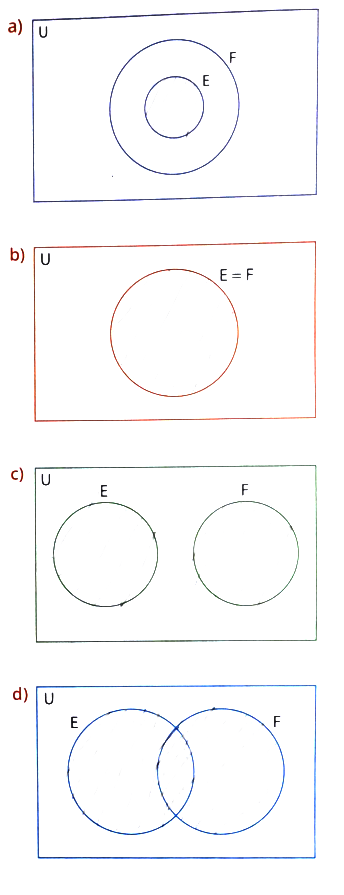
\includegraphics[width=1.1\linewidth]{6FMA52_imagens/imagem1} \columnbreak
    			\item Hachurar $A \cup B$. \\
    			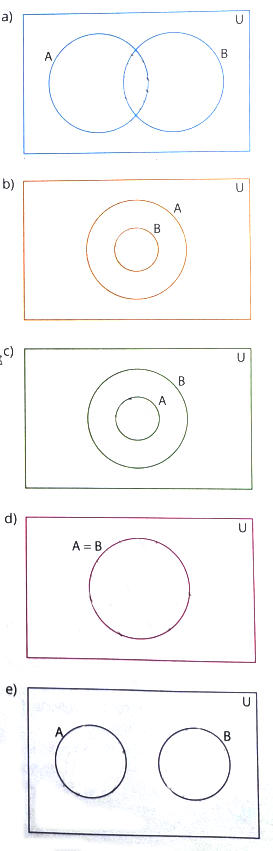
\includegraphics[width=1\linewidth]{6FMA52_imagens/imagem2} \newpage
    			\item Dados $H, I$ e $J$, apresentar $H \cup I \cup J$:
    			\begin{enumerate}[a)]
    				\item $H = \{2, 4\}, I = \{4, 6\}, \\ J = \{6, 8\}$ 
    				\item $H = \{\{8\},\{9\}\}, \\ I = \{\{8\}, 9\}, J = \{8, 9\}$
    				\item $H = \{1\}, I = \varnothing, J = \{1, 2\}$
    				\item $H = \{3\}, I = \{5\}, J = \{7\}$
    				\item $H = \{10, 11\}, I = \{10\}, \\ J = \{11\}$
    				\item $H = \{15, 16, 17\}, \\ I = \{12, 13\}, J = \{14\}$
    				\item $H = \varnothing, I = \{6, 7, 8\}, J = \varnothing$
    				\item $H = \varnothing, I = \varnothing, J = \varnothing$ \\\\\\\\\\\\\\\\\\\\\\\\\\\\\\\\\\\\\\\\\\\\\\\\
    			\end{enumerate}
    			\item Dados $X = \{5, 6, 8\}, Y = \{7, 8, 9\}$ e $Z = \{4, 7, 9\}$, apresentar:
    			\begin{enumerate}[a)]
    				\item $X \cap (Y \cup Z)$
    				\item $(X \cap Y) \cup Z$
    				\item $X \cup (Y \cap Z)$
    				\item $(X \cup Y) \cap Z$
    				\item $(X \cap Y) \cup (X \cap Z)$
    				\item $(X \cup Z) \cap (Y \cup Z)$
    				\item $(X \cup Y) \cap (X \cup Z)$
    				\item $(X \cap Z) \cup (Y \cap Z)$
    				\item $X \cup Y \cup Z$
    				\item $X \cap Y \cap Z$
    				\item $(X \cup Y \cup Z) \cap X$
    				\item $(X \cap Y \cap Z) \cup X$
    			\end{enumerate}
    		\end{enumerate}
    		$~$ \\ $~$ \\ $~$ \\ $~$ \\ $~$ \\ $~$ \\ $~$ \\ $~$ \\ $~$ \\ $~$ \\ $~$ \\ $~$ \\ $~$ \\ $~$ \\ $~$ \\ $~$ \\ $~$ \\ $~$ \\ $~$ \\ $~$ \\ $~$ \\ $~$
	\end{multicols}
\end{document}